% Gravity Research Foundation 2027 essay, as submitted on 2026-09-11.
% Format per competition rules: 12pt, double-spaced, single column, 1-inch margins,
% at most 10 pages of body; title page and reference pages are extra.
\documentclass[12pt]{article}
\usepackage[margin=1in]{geometry}
\usepackage{setspace}
\usepackage{amsmath,amssymb}
\usepackage{microtype}
\usepackage[hidelinks]{hyperref}
\usepackage{tikz}
\usetikzlibrary{arrows.meta,positioning,calc}
\makeatletter
\renewcommand\section{\@startsection{section}{1}{\z@}{-1.4ex plus -0.4ex minus -0.2ex}{0.7ex plus 0.1ex}{\normalfont\large\bfseries}}
\@secpenalty=0
\def\@afterheading{\@nobreaktrue\everypar{\if@nobreak\@nobreakfalse\clubpenalty\z@\if@afterindent\else{\setbox\z@\lastbox}\fi\else\clubpenalty\@clubpenalty\everypar{}\fi}}
\makeatother
\raggedbottom
\widowpenalty=150
\clubpenalty=150
\pagestyle{plain}
\setlength{\parskip}{0pt}
\setlength{\parindent}{1.5em}
\newcommand{\Gab}{G_{ab}}
\newcommand{\Tab}{T_{ab}}
\begin{document}

\thispagestyle{empty}
\begin{center}
\vspace*{2.5cm}
{\LARGE\bfseries The Price of Agreement:\\[0.4em] Gravity as the Geometry of Consensus\par}
\vspace{2cm}
{\large Bernhard Mueller\par}
\vspace{0.6em}
Pragma Research Inc.\par
\vspace{0.4em}
{\small Chiang Mai\par Thailand\par}
\vspace{0.6em}
Corresponding author: Bernhard Mueller, \texttt{bernhard@floatingpragma.ai}\par
\vspace{2cm}
Submission date: September 11, 2026\par
\vspace{1.5cm}
{\small Essay written for the Gravity Research Foundation 2027 Awards for Essays on Gravitation\par}
\end{center}
\vfill
\begin{singlespace}
\noindent\textbf{Abstract.}
To a trained physicist this essay's starting point may sound absurd: it assumes no spacetime. Physics normally begins there, and gravity is the one thing showing this cannot be right, since gravity is the geometry the fields are written on and cannot be added as one more field. The essay starts from computation, finite observers repairing disagreements until they agree, and from there uses only long-known arguments: a Bombelli--Lee--Meyer--Sorkin causal set from read-after-write dependence, rank three from the slowest repair mode, Jaynes maximum-entropy fixed points with a Bisognano--Wichmann clock on every boundary. These are the inputs Jacobson's derivation takes as given, so Einstein's equation follows. Every finite step is machine-checked in Lean \cite{ophflagship,ophrepo}.
\end{singlespace}
\clearpage
\setcounter{page}{1}
\begin{doublespace}

\section*{A small thing to fix}

Quantum field theory describes three of the four forces to a precision that embarrasses the instruments, and it describes the fourth not at all. Gravity is weak, it is universal, and it is carried, if it is carried by anything, by a massless particle of spin two. The obvious repair is to write that particle down on the flat spacetime everything else lives on and let the machinery run.

The machinery does not run, and the way it fails is instructive. A massless spin-two field that couples to energy must couple to its own energy, and when Deser followed that requirement to its end in 1970 the field had eaten its background: the consistent self-coupled theory is general relativity, with the flat spacetime it started on gone \cite{deser1970}. Push on and quantize anyway, and pure gravity develops an incurable divergence at two loops \cite{goroffsagnotti1986}. Try instead to let the graviton emerge as a bound state of ordinary fields on a fixed spacetime, and Weinberg and Witten showed in 1980 that no Lorentz-covariant theory with a covariant conserved stress tensor can produce one \cite{weinbergwitten1980}. Every route that keeps the rest of physics and adds gravity to it hits the same wall: gravity is the geometry the other fields are written on. A field theory needs a metric to say what is local, what is causal, what a particle is, and what the vacuum is, and the thing being added is that metric.

So the small fix is no fix. Gravity is geometric, and that is why every attempt to make it a field on a stage fails: it is the stage. If it cannot be added to the foundations, the foundations have to be rebuilt in a way that has no geometry in them to begin with, so that the geometry, and with it gravity, comes out at the end. That is what this essay does. The starting point is computation: finite observers with bounded memory and a few ports each, obliged to agree with their neighbours about what they jointly see. The route from there to Einstein's equation uses arguments that have been in the literature for decades; what is new is the order they are put in.

\section*{Three accessories not in the box}

The air above your kitchen table has a horizon. Pick a point in it and a direction, and imagine an observer accelerating through that point in that direction for long enough. A surface forms behind it that no signal will cross in its direction, a Rindler horizon, and Unruh showed in 1976 that the observer reads the vacuum beyond that surface as warm, at a temperature proportional to the acceleration \cite{unruh76}. In 1995 Ted Jacobson took this seriously in every direction at once \cite{jacobson95}. Give each such horizon an entropy proportional to its area and require that the heat crossing it obey Clausius, $\delta Q = T\,dS$, at every point and along every direction. The geometry then has no freedom left. It has to curve in the one way that keeps the accounts straight, and that curvature is $\Gab + \Lambda g_{ab} = 8\pi G\,\Tab$, which is Einstein's equation arrived at by accountancy. In 2016 Jacobson compressed the premise to one clause, stationarity of the entanglement entropy of every small ball at fixed volume \cite{jacobson16}. Verlinde and Padmanabhan later read the same thermodynamics into Newton's law and into a wide class of gravity theories \cite{verlinde2011,padmanabhan2010}.

The derivation works perfectly provided you have bought three accessories that are not in the box. Nothing in it says why a horizon's entropy should count area, why a surface that is an accident of one observer's acceleration should have a temperature, or why the state of the world should be one in which entropy is stationary on every small region in every direction at all times. Jacobson calls the last of these a hypothesis, which is the polite word. Eling, Guedens, and Jacobson worked out what happens when it fails: the equation of state acquires dissipative terms and Einstein's equation stops being exact \cite{elingguedensjacobson2006}. The equilibrium carries the whole weight of the argument, and nothing in the argument holds the world in it. The derivation reasons about a clock, a thermometer, and an equilibrium that nobody has located on the board.

The claim of this essay is that all three are on the board of one particular device, a network of finite observers who must agree. The area law is the number of connections a cut severs. The temperature is the clock a finite record carries with it whether it asked for one or not. The equilibrium is what agreement means. The material comes from the Observer Patch Holography programme, which checks its mathematics in the Lean prover \cite{ophflagship,ophrepo}.

\section*{What an observer is}

An observer here holds a bounded amount of state, reads the outside through finitely many ports, writes records that later moves may not touch, and shares boundaries with neighbours whose records must agree with its own where they overlap, because two accounts of one shared fact cannot both stand. The programme assumes three things \cite{ophflagship}. Observers form a federation on a spherical support, each with twelve ports at the vertices of an icosahedron, joined to neighbours through seams, a seam being two ports routed to each other. Observers agree: any datum two of them jointly read means the same to both, on every overlap. Whatever agreement leaves unconstrained is maximally random. The third assumption is Jaynes's maximum-entropy principle \cite{jaynes1957} promoted from advice to statisticians to a law of nature.

None of the three assumptions mentions space, time, fields, or gravity. The only dynamics is repair. When two ports across a seam disagree, the patches rewrite themselves from what they share until they do not, every accepted repair lowers a mismatch potential, and on a finite network the process ends. On a federation of $81{,}920$ patches the potential descends under sixteen different asynchronous schedules and all sixteen land on the same public normal form \cite{ophrepo}. That schedule independence is what objectivity amounts to here.

\section*{Where before and after come from}

With no global timeline, ``before'' can only mean dependence. A record written after reading another record depends on it, and the transitive closure of authenticated read-after-write dependence is a strict partial order on records. Lamport saw in 1978 that this is the only time a distributed system has \cite{lamport1978}; he was thinking about computers that had to agree on the order of things without being able to see one another, which is the universe's problem with better documentation. In the observer network the relation is machine-checked to be irreflexive, transitive, and locally finite \cite{ophflagship}, and a locally finite partial order is the object Bombelli, Lee, Meyer, and Sorkin proposed in 1987 as the discrete precursor of spacetime \cite{bombelli1987}, and in a distinguishing spacetime the causal order fixes the metric up to a conformal factor, with a volume element fixing the rest \cite{malament1977,hawkingkingmccarthy1976}.

Two records that do not depend on each other are incomparable in the order, and incomparable is spacelike. Observers fail to agree on simultaneity because simultaneity was never in the record; there is no ``now'' on the board. What the observer does have is a height, the length of the longest chain of dependencies ending at a record, and Lean proves that height strictly increases along the order and that a chain attaining it exists.

\section*{Where three plus one comes from}

The spatial directions come from the ports. Twelve ports on an icosahedron carry the rotation group $A_5$, and the twelve-dimensional space of port readings splits as
\begin{equation}
P_{12}\;\cong\;\mathbf{1}\oplus\mathbf{3}\oplus\mathbf{3}'\oplus\mathbf{5},
\end{equation}
an exact decomposition with no repeated summand. Repair acts on this split as a low-pass filter. The uniform seam-mean rule is $T = I - L/60$ with $L$ the icosahedral Laplacian, so each band fades at its own rate per step, $(55+\sqrt5)/60$ for one triplet, $9/10$ for the quintet, and $(55-\sqrt5)/60$ for the other triplet. Content that has faded before a second observer can compare it anchors nothing, so only the slowest band lasts, and its rank is three. The normalized response kernel converges to $4P_{\mathrm{slow}}$, a projector of rank three, and the integer records embed densely in the three-dimensional Euclidean space it defines \cite{ophflagship}. A struck bell ends on one note for the same reason: the other modes rang down first.

Adjoin the height axis to that space and write the obvious quadratic form, $Q(t,x) = t^2 - g(x,x)$. It has one positive and three negative directions, and the unit spatial directions are its future null rays, so the sphere of port directions, the celestial sphere, and the edge of the light cone are the same set. A separate theorem fixes the cone: a closed convex pointed cone invariant under the icosahedral rotations and under boosts along one axis is the Lorentz cone, and a time orientation picks the future half \cite{ophEinstein}.

On a supplied population of $q^3$ golden-ratio sites with a complete-neighbour read law, the provenance order is proved equal to a layered order with an exact cone sandwich, and finite runs read a Myrheim--Meyer dimension of $4.09$ at $q=55$ against $3.02$ and $2.00$ for two- and one-dimensional control populations, and an interval ordering fraction of $0.093$ against the flat four-dimensional value $1/10$ \cite{ophEinstein}.

\begin{figure}[t]
\centering
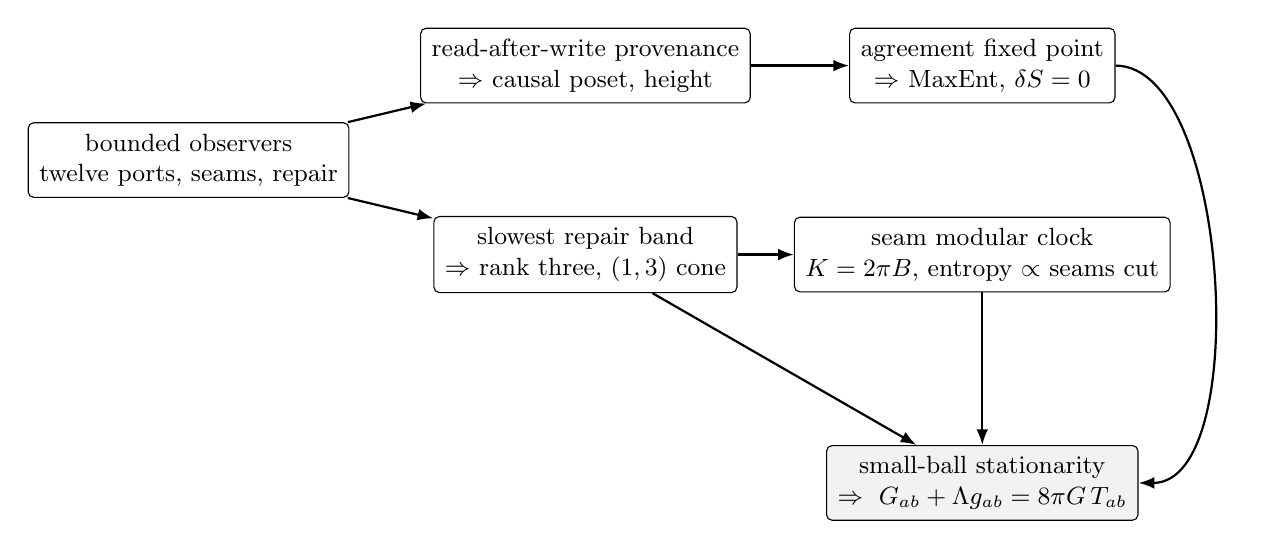
\begin{tikzpicture}[x=0.9cm,y=1cm,
  box/.style={draw,rounded corners=2pt,align=center,font=\small,inner sep=4pt,minimum height=0.9cm},
  arr/.style={-{Latex[length=2mm]},thick}]
\node[box] (obs) at (0,0) {bounded observers\\twelve ports, seams, repair};
\node[box] (ord) at (5.6,1.2) {read-after-write provenance\\$\Rightarrow$ causal poset, height};
\node[box] (dim) at (5.6,-1.2) {slowest repair band\\$\Rightarrow$ rank three, $(1,3)$ cone};
\node[box] (eq) at (11.2,1.2) {agreement fixed point\\$\Rightarrow$ MaxEnt, $\delta S = 0$};
\node[box] (mod) at (11.2,-1.2) {seam modular clock\\$K = 2\pi B$, entropy $\propto$ seams cut};
\node[box,fill=black!5] (ein) at (11.2,-4.1) {small-ball stationarity\\$\Rightarrow\ \Gab+\Lambda g_{ab}=8\pi G\,\Tab$};
\draw[arr] (obs) -- (ord);
\draw[arr] (obs) -- (dim);
\draw[arr] (ord) -- (eq);
\draw[arr] (dim) -- (mod);
\draw[arr] (eq.east) to[out=0,in=0,looseness=0.7] (ein.east);
\draw[arr] (mod) -- (ein);
\draw[arr] (dim) -- (ein);
\end{tikzpicture}
\caption{From bounded observers to the field equation. The left half is finite mathematics; the right half supplies the three inputs Jacobson's derivation takes as given.}
\end{figure}

\section*{Why agreement is entropy stationarity}

Take one seam and the repair that settles it. The repair is handed some quantities the two neighbours have fixed between them and some they have not, and the third assumption is its merge policy: keep every settled quantity as it stands and regenerate everything else from the reference. That instruction is a conditional projection, a recovery map on the collar around a region \cite{petz1988}, and it is idempotent, it preserves the reference, and for any state $p$ and reference $\pi$ it contracts relative entropy, $D(pP\,\|\,\pi)\le D(p\,\|\,\pi)$. The mean entropy production of one step equals that descent, so the second law is the Jensen shadow of the identity $\langle e^{-\sigma}\rangle = 1$ \cite{ophflagship}.

A state of agreement is a state that repair leaves where it found it, a fixed point. The fixed points of a reference-preserving conditional projection are the maximum-entropy states compatible with what has been settled, the Gibbs states of the constraints, by the finite Pythagorean identity of information geometry, which is proved in Lean for the finite kernel. So ``the observers agree'' and ``the entropy is stationary under every admissible variation'' describe one state. A state that could raise its entropy at first order without breaking a settled constraint is a state that repair would move, and a state that repair would move is one the neighbours have not finished arguing about. Jacobson's entanglement equilibrium is the definition of consensus.

Seen from inside, the boundary of a region is the set of seams its observers cannot read past, which is what a Rindler horizon is for the accelerating observer. Every finite state ships with a clock, whether or not one was ordered: the modular flow of Tomita and Takesaki with generator $K=-\log\rho$ \cite{takesaki1970}, the one reshuffling of an observer's questions that keeps its bookkeeping consistent. Bisognano and Wichmann proved that for a wedge of the vacuum this flow is the Lorentz boost, $K=2\pi B$, and the $2\pi$ is the Unruh temperature \cite{bw76}. The temperature Jacobson had to import was in the state all along. In the finite network the modular generator on a cap splits as $K = 2\pi B + Z$, with $B$ the boost of the seam and $Z$ the part that commutes with the records, and the first-law identity $S(p)-S(\tau)=\langle K\rangle_p-\langle K\rangle_\tau - D(p\|\tau)$ is exact. Reading $B$ as a physical boost and $2\pi$ as a laboratory temperature is the one place where the construction consumes a physical map.

The area law needs no gravity. A cut through a region's boundary severs a definite number of seams. Nothing is printed on a port that would make one join wider than another, so the entropy of a cut counts seams, each worth the same, and a count of seams on a surface is an area in the only unit the surface has. Bekenstein's quarter of the horizon area in Planck units \cite{bekenstein1973}, read backwards, is the exchange rate, and Newton's constant is the number of square metres per record.

\section*{The equation}

With the three accessories installed the rest is Jacobson's small-ball calculation. Fix a small causal diamond of radius $\ell$ around any event and vary the state at fixed volume. The generalized entropy is the entropy of the contents plus the seam count of the boundary,
\begin{equation}
S_{\mathrm{gen}} = S_{\mathrm{bulk}} + \frac{A}{4G},
\end{equation}
and at an agreement fixed point its first variation vanishes. By the first law with $K=2\pi B$ the bulk term is $\delta S_{\mathrm{bulk}} = (8\pi^2\ell^4/15)\,\delta\langle T_{00}\rangle$, and the area term at fixed volume is $\delta A = -(4\pi\ell^4/15)\,\delta(G_{00}+\Lambda g_{00})$. Every power of $\ell$ cancels, both fifteens cancel, and what is left is
\begin{equation}
\Gab\,k^ak^b = 8\pi G\,\Tab\,k^ak^b
\end{equation}
for every null $k$. The $8\pi$ that every textbook writes in front of Newton's constant without comment is the ratio of two elementary integrals over a ball. Null values determine a symmetric tensor up to a multiple of the metric, a finite linear-algebra fact proved in Lean; the contracted Bianchi identity and conservation of the stress tensor then force that multiple to be constant, which is the cosmological term, and the full equation $\Gab+\Lambda g_{ab}=8\pi G\,\Tab$ follows on any $C^3$ Lorentzian four-manifold from the null balance and the Ward identity \cite{ophflagship,ophEinstein}.

Vacuum energy is proportional to the metric, and the metric is blind along null rays, $g_{ab}k^ak^b=0$, so the one direction light rays cannot see is the direction the vacuum's energy points in. The small-ball argument is built out of horizons, horizons are made of rays, and rays are blind to $\Lambda$, which is why every local calculation of it was doomed before it started. What fixes it is a count no small region contains, the total record capacity $N$ of the horizon around an observer. On the fixed-capacity branch the dictionary is $\Lambda\,\ell_P^2 = 3\pi/N$, and with $N$ near $3.3\times10^{122}$ records the constant lands within one percent of the measured $1.09\times10^{-52}\,\mathrm{m}^{-2}$ \cite{ophflagship}. This is the capacity re-expressed in the vacuum coordinate, and the programme says so. The branch has a kill condition: fixed capacity implies a dark-energy equation of state of $w=-1$, and a firm DESI measurement of $w\neq-1$ kills it \cite{desidr2}.

\section*{What gravity is}

Gravity is what a settled network of observers looks like from a distance. The metric describes the stable causal relation among repaired records, modular flow describes how a patch reads change, and entropy stationarity fixes the response that keeps local accounts compatible \cite{ophflagship}. Put matter somewhere, meaning a bounded pattern of records that has to be re-asserted on every cycle against the seams around it, and those seams are spent faster. Mass is that standing cost. It resists a push and it bends the geometry around it, and those are one entry in one ledger read twice, once as a price and once as a source. MICROSCOPE spent two and a half years in orbit checking that the two readings agree to a part in $10^{15}$ \cite{microscope2022}, which they do.

There is no way to opt out of agreement, and that is the whole reason gravity is inevitable. An observer that reads its neighbours through finitely many ports and must not contradict them has records that generate a causal order, a slow band of rank three, a modular clock on every seam, and fixed points at maximum entropy. A world in which those hold on every seam is a world in which every small ball obeys the null balance, and there is nothing anybody can do about it, including the ball. This is also why the small fix of the first section could never work. The field theorist's spacetime is the agreed state of a network of observers, and asking it to carry one more quantum field is asking a settled account to contain, as an entry, the fact of its own settlement.

\section*{What is proved and what is identified}

The chain has one seam in it, and it belongs here, stated once. On the finite side everything is a theorem or an exact certificate: the partial order, the height, the band split, the rank-three Gram identity, the $(1,3)$ carrier, the first-law and fluctuation identities, the Gibbs fixed point, the cap Clausius inequality, null tomography, the small-ball arithmetic, and the tensor completion from a realized null balance and Ward identity, in a Lean library with no admitted propositions in the reported dependency closure \cite{ophrepo}. The cone-selection theorem and the count-volume limits are analytic proofs in the companion paper. The passage from that finite world to a smooth curved spacetime is a reconstruction. It requires that the physical events be the records, that the physical clock be the modular parameter with its $2\pi$, that a variation of the seam count be a variation of area, that count calibrate volume, and that one common refinement family realize the event, modular, stress, and entropy premises together. The programme names these maps and states that no result discharges them \cite{ophflagship}. They are the identifications Jacobson's derivation makes when it calls a Rindler wedge's modular Hamiltonian a boost and its entanglement entropy an area. Here they are supplied by the definition of an observer.

\section*{Four buildings}

The pieces were held in four buildings whose occupants did not visit each other: Jaynes in 1957, Lamport in 1978, Bombelli, Lee, Meyer, and Sorkin in 1987, and Jacobson in 1995. Read together they say that a finite observer obliged to agree with its neighbours has gravity whether it likes it or not. Jacobson ended the abstract of his 1995 paper by remarking that it may be no more appropriate to quantize the Einstein equation than to quantize the wave equation for sound in air. Sound needs air, and an equation of state needs a gas that has settled down. What the gas is made of here is observers, and what settling down means for them is agreement.

\end{doublespace}
\clearpage
\begin{singlespace}
\begin{thebibliography}{99}
\small

\bibitem{unruh76}
W.~G.~Unruh, ``Notes on black-hole evaporation,'' \emph{Phys.\ Rev.\ D} \textbf{14}, 870--892 (1976).

\bibitem{jacobson95}
T.~Jacobson, ``Thermodynamics of spacetime: The Einstein equation of state,'' \emph{Phys.\ Rev.\ Lett.} \textbf{75}, 1260--1263 (1995).

\bibitem{jacobson16}
T.~Jacobson, ``Entanglement equilibrium and the Einstein equation,'' \emph{Phys.\ Rev.\ Lett.} \textbf{116}, 201101 (2016).

\bibitem{verlinde2011}
E.~Verlinde, ``On the origin of gravity and the laws of Newton,'' \emph{J.\ High Energy Phys.} \textbf{2011}(4), 29 (2011).

\bibitem{padmanabhan2010}
T.~Padmanabhan, ``Thermodynamical aspects of gravity: new insights,'' \emph{Rep.\ Prog.\ Phys.} \textbf{73}, 046901 (2010).

\bibitem{elingguedensjacobson2006}
C.~Eling, R.~Guedens, and T.~Jacobson, ``Nonequilibrium thermodynamics of spacetime,'' \emph{Phys.\ Rev.\ Lett.} \textbf{96}, 121301 (2006).

\bibitem{ophflagship}
B.~Mueller, A.~Osika, M.~Poneder, K.~Xue, B.~Cassie, P.~Nguyen, J.~Kim, D.~Matscheko, J.~Hill, W.~T.~Glynn, M.~A.~Visser, K.~A.~Anirudha, and B.~de~La~Fourni\`ere, ``Finite observer consensus as a reconstruction principle: normal forms, the Standard Model Lie type, and a route to the Einstein field equation,'' PhilPapers record MUEFOC (2026). \url{https://philpapers.org/rec/MUEFOC}

\bibitem{ophrepo}
FloatingPragma, \emph{Observer Patch Holography: Lean library, exact code receipts, finite certificates, and scientific claim registries} (2026). \url{https://github.com/FloatingPragma/observer-patch-holography}

\bibitem{ophEinstein}
B.~Mueller, A.~Osika, M.~Poneder, K.~Xue, P.~Nguyen, M.~A.~Visser, D.~Matscheko, and B.~de~La~Fourni\`ere, ``Recovering observer spacetime and Einstein dynamics from overlap consistency,'' companion paper in \cite{ophrepo}, directory \texttt{paper/} (2026).

\bibitem{deser1970}
S.~Deser, ``Self-interaction and gauge invariance,'' \emph{Gen.\ Relativ.\ Gravit.} \textbf{1}, 9--18 (1970).

\bibitem{weinbergwitten1980}
S.~Weinberg and E.~Witten, ``Limits on massless particles,'' \emph{Phys.\ Lett.\ B} \textbf{96}, 59--62 (1980).

\bibitem{goroffsagnotti1986}
M.~H.~Goroff and A.~Sagnotti, ``The ultraviolet behavior of Einstein gravity,'' \emph{Nucl.\ Phys.\ B} \textbf{266}, 709--736 (1986).

\bibitem{jaynes1957}
E.~T.~Jaynes, ``Information theory and statistical mechanics,'' \emph{Phys.\ Rev.} \textbf{106}, 620--630 (1957).

\bibitem{lamport1978}
L.~Lamport, ``Time, clocks, and the ordering of events in a distributed system,'' \emph{Commun.\ ACM} \textbf{21}(7), 558--565 (1978).

\bibitem{bombelli1987}
L.~Bombelli, J.~Lee, D.~Meyer, and R.~D.~Sorkin, ``Space-time as a causal set,'' \emph{Phys.\ Rev.\ Lett.} \textbf{59}, 521--524 (1987).

\bibitem{malament1977}
D.~B.~Malament, ``The class of continuous timelike curves determines the topology of spacetime,'' \emph{J.\ Math.\ Phys.} \textbf{18}, 1399--1404 (1977).

\bibitem{hawkingkingmccarthy1976}
S.~W.~Hawking, A.~R.~King, and P.~J.~McCarthy, ``A new topology for curved space--time which incorporates the causal, differential, and conformal structures,'' \emph{J.\ Math.\ Phys.} \textbf{17}, 174--181 (1976).

\bibitem{petz1988}
D.~Petz, ``Sufficiency of channels over von Neumann algebras,'' \emph{Q.\ J.\ Math.\ Oxford} \textbf{39}, 97--108 (1988).

\bibitem{takesaki1970}
M.~Takesaki, \emph{Tomita's Theory of Modular Hilbert Algebras and its Applications}, Lecture Notes in Mathematics 128 (Springer, Berlin, 1970).

\bibitem{bw76}
J.~J.~Bisognano and E.~H.~Wichmann, ``On the duality condition for quantum fields,'' \emph{J.\ Math.\ Phys.} \textbf{17}, 303--321 (1976).

\bibitem{bekenstein1973}
J.~D.~Bekenstein, ``Black holes and entropy,'' \emph{Phys.\ Rev.\ D} \textbf{7}, 2333--2346 (1973).

\bibitem{microscope2022}
P.~Touboul et al.\ (MICROSCOPE Collaboration), ``MICROSCOPE mission: Final results of the test of the equivalence principle,'' \emph{Phys.\ Rev.\ Lett.} \textbf{129}, 121102 (2022).

\bibitem{desidr2}
DESI Collaboration, ``DESI DR2 results II: Measurements of baryon acoustic oscillations and cosmological constraints,'' arXiv:2503.14738 (2025).

\end{thebibliography}
\end{singlespace}
\end{document}
